%%%%%%%%%%%%%%%%%%%%%%%%%%%%%%%%%%%%%%%%%%%%%%%%%%%%%%%%%%%%%%%%%%%%%%%%%%%%%%%
%
% Tommy P. Keane
% Master of Science Thesis
% Department of Electrical and Microelectronic Engineering
% Rochester Institute of Technology
%
% April 2011
%
%
%
% Funded By: Lenel Systems Inc., A UTC Fire & Security Corporation
%
% Algorithm Intellectual Property Owned By: Lenel Systems Inc.
%
%
% http://www.tommypkeane.com
%
%%%%%%%%%%%%%%%%%%%%%%%%%%%%%%%%%%%%%%%%%%%%%%%%%%%%%%%%%%%%%%%%%%%%%%%%%%%%%%%

%%%%%%%%%%%%%%%%%%%%%%%%%%%%%%%%%%%%%%%%%%%%%%%%%%%%%%%%%%%%%%%%%%%%%%%%%%%%%%%
%
% CHAPTER 4
%
% SECTION 2: Near-Affine Views
%
%%%%%%%%%%%%%%%%%%%%%%%%%%%%%%%%%%%%%%%%%%%%%%%%%%%%%%%%%%%%%%%%%%%%%%%%%%%%%%%


%%%%%%%%%%%%%%%%%%%%%%%%%%%%%%%%%%%%%%%%%%%%%%%%%%%%%%%%%%%%%%%%%%%%%%%%%%%%%%%
% BEGIN DOCUMENT

The affine related views of the previous section are entirely unrealistic, as stated, but in making a slow transition to evaluate the algorithm in realistic scenarios, views with near-affine relations can be generated in reality. In Figure \ref{ArtGallery4Images5} the views are not affine related, but being that there is only a slight rotation between the views (the right view's camera was rotated only a few degrees along the horizontal axis in-line with the camera centers) there is almost no occlusion or parallax disparity, and there is very little depth variation in the objects between the views. While all these characteristics (occlusion, parallax, and depth) do exist in the views, they are minimal enough that they can be ignored and an affine homography should perform quite well in registering the views.

Applying the WFMI algorithm to the views from Figure \ref{ArtGallery4Images5} produces the automatically generated panorama in Figure \ref{ArtGallery4Stitched5} with a manually generated panorama presented in Figure \ref{ArtGallery4StitchedManual5}. A second set of views for the same scene is shown in Figure \ref{ArtGallery4Images7}, with a third set of views in Figure \ref{ArtGallery4Images8}. For these two sets, the difference is that the angle of rotation of the second camera was much larger than the previous view(s). This creates more and more depth distortion, and less and less overlap. Also, because of the nature of the scene, the more rotation there is, the less the objects overwhelm the scene structure and the repeated pattern (low entropy) of the brick floor begins to be the majority of the scene content. This makes registration extremely difficult, but again as the WFMI algorithm is structural in nature, it is shown in the two alternate sets of views that the registration still provides a very accurate estimate beyond the near-affine scenarios and in the presence of very low entropy.

These results show that the algorithm does function for real scenes with real scene content, but these views were generated under restrictions on parallax and occlusion, despite the robustness of the algorithm in the face of entropy and overlap concerns. The next section is the true test of the algorithm as all the views are not only susceptible to low entropy and minimal overlaps, but there is often extreme amounts of parallax disparity and occlusion variation for objects between the views.

% ART GALLERY 4 - 005
\begin{figure}
\centering
\subfigure{ 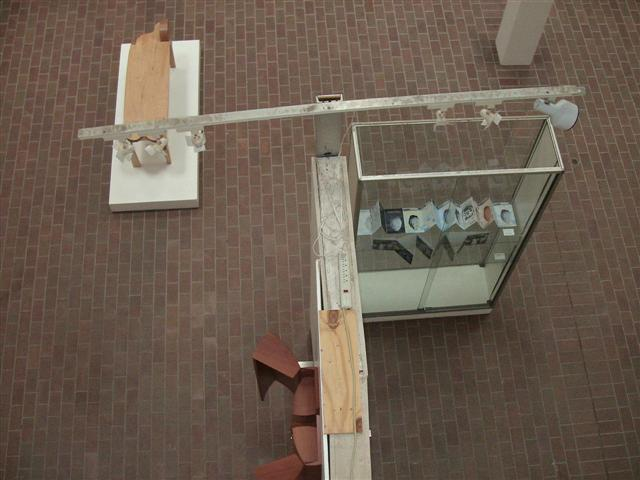
\includegraphics[width=.4\textwidth]{AGS4L005} \label{AGS4L005} }
\subfigure{ 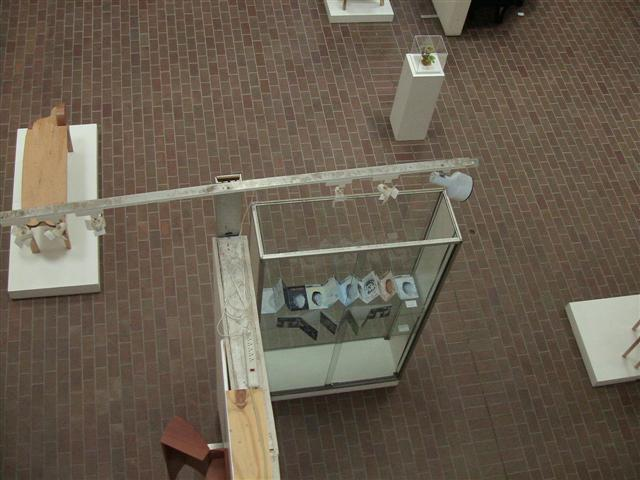
\includegraphics[width=.4\textwidth]{AGS4R005} \label{AGS4R005} }
\caption{Art Gallery Scene (a) Left View, (b) Right View}
\label{ArtGallery4Images5}
\end{figure}

\begin{figure}
\centering
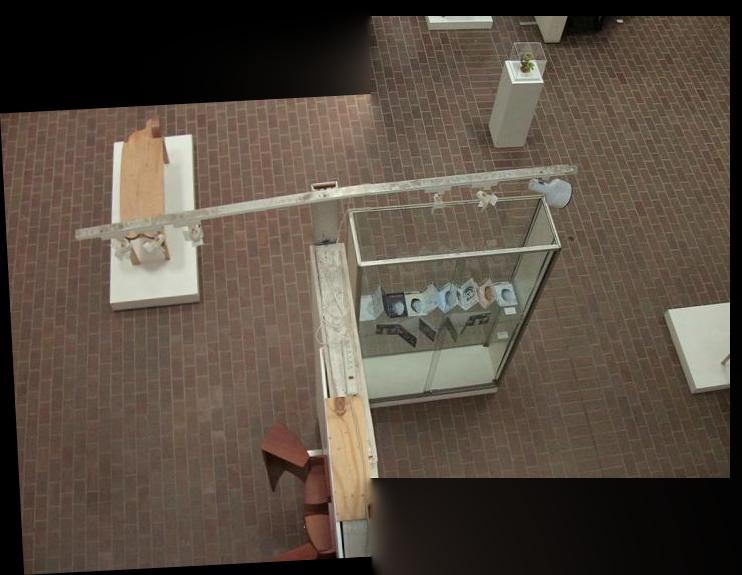
\includegraphics[width=1\textwidth]{AGS4SP005005}
\caption{Art Gallery Views Blended}
\label{ArtGallery4Stitched5}
\end{figure}

\begin{figure}
\centering
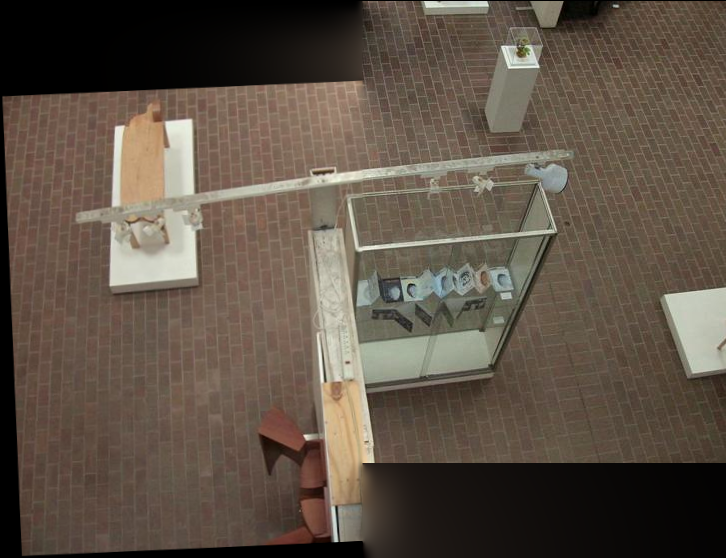
\includegraphics[width=1\textwidth]{AGS4SP005ManAff}
\caption{Art Gallery Views Blended Manually (Affine)}
\label{ArtGallery4StitchedManual5}
\end{figure}


% ART GALLERY 4 - 007
\begin{figure}
\centering
\subfigure{ 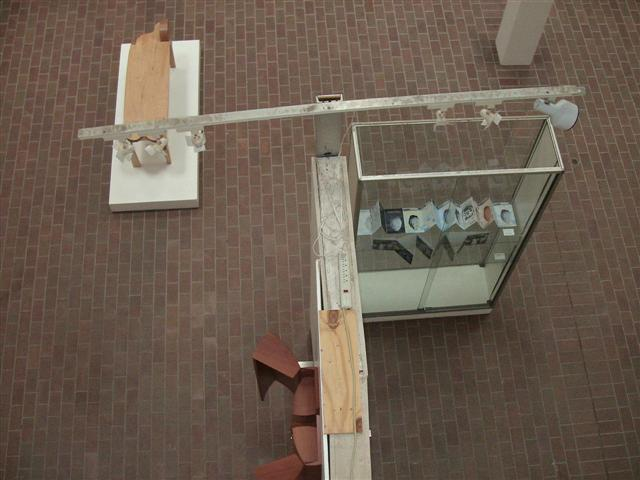
\includegraphics[width=.4\textwidth]{AGS4L007} \label{AGS4L007} }
\subfigure{ 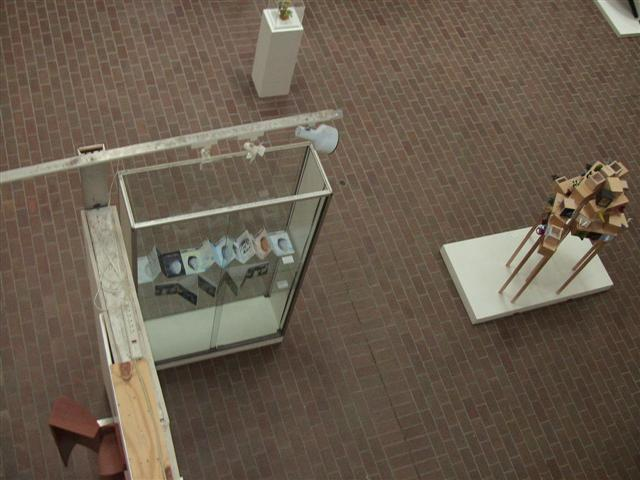
\includegraphics[width=.4\textwidth]{AGS4R007} \label{AGS4R007} }
\caption{Art Gallery Scene (Modest Angle) Views (a) Left View, (b) Right View}
\label{ArtGallery4Images7}
\end{figure}

\begin{figure}
\centering
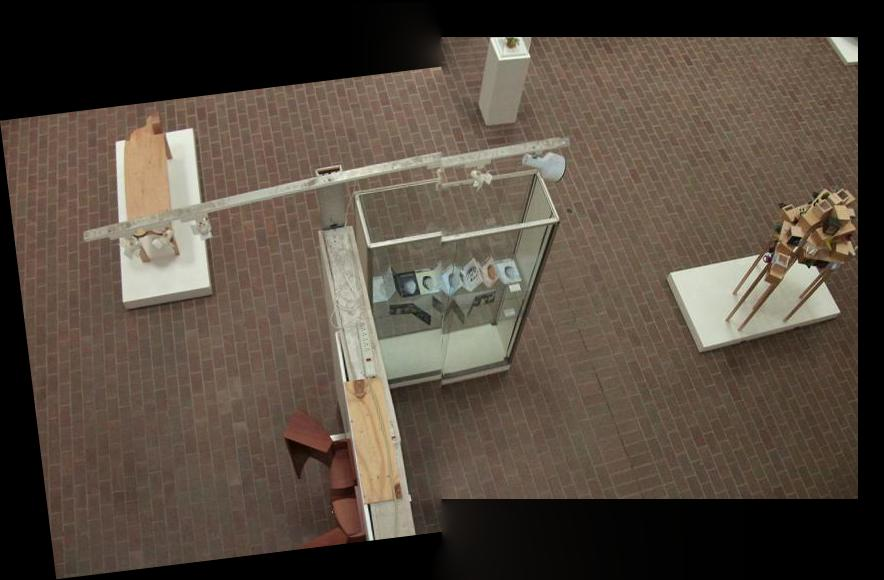
\includegraphics[width=1\textwidth]{AGS4SP007007}
\caption{Art Gallery (Modest Angle) Views Blended}
\label{ArtGallery4Stitched7}
\end{figure}


% ART GALLERY 4 - 008
\begin{figure}
\centering
\subfigure{ 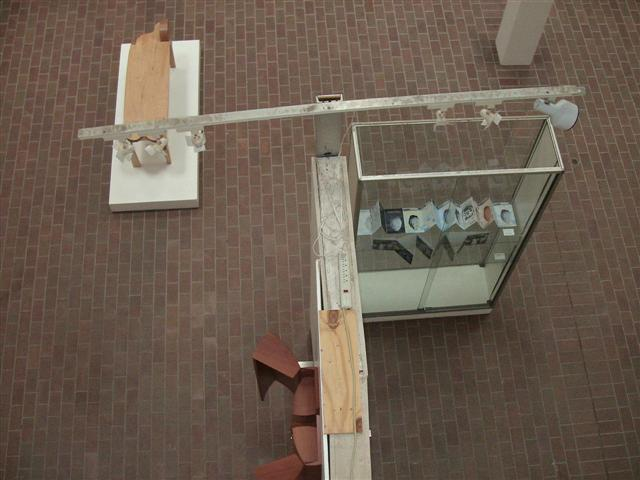
\includegraphics[width=.4\textwidth]{AGS4L008} \label{AGS4L008} }
\subfigure{ 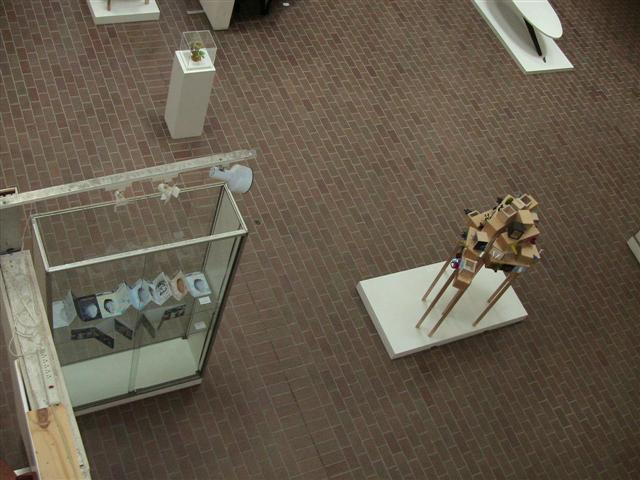
\includegraphics[width=.4\textwidth]{AGS4R008} \label{AGS4R008} }
\caption{Art Gallery (Large Angle) Views (a) Left View, (b) Right View}
\label{ArtGallery4Images8}
\end{figure}

\begin{figure}
\centering
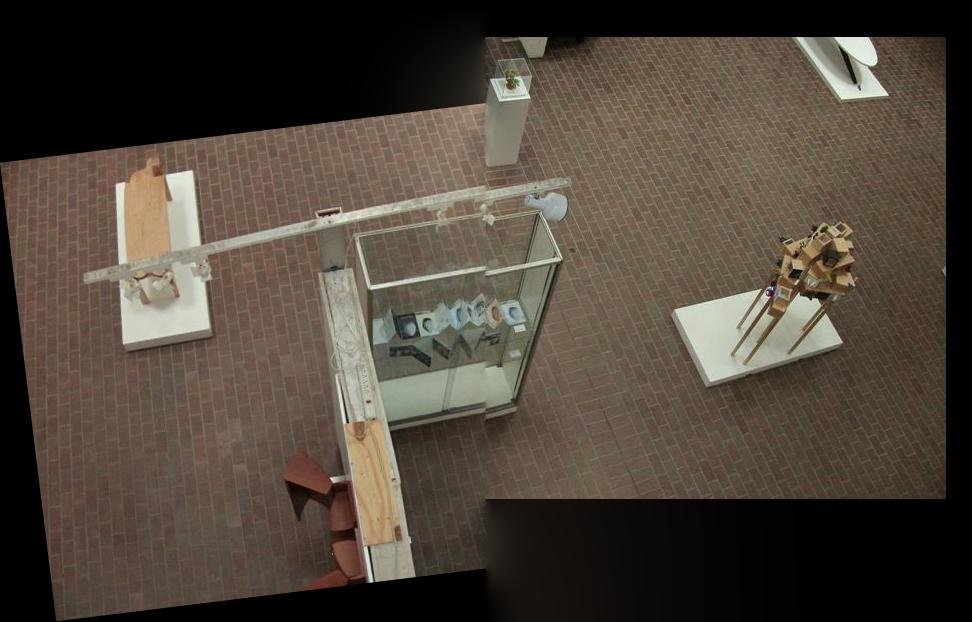
\includegraphics[width=1\textwidth]{AGS4SP008008}
\caption{Art Gallery (Large Angle) Views Blended}
\label{ArtGallery4Stitched8}
\end{figure}



%%%%%%%%%%%%%%%%%%%%%%%%%%%%%%%%%%%%%%%%%%%%%%%%%%%%%%%%%%%%%%%%%%%%%%%%%%%%%%%
% END OF DOCUMENT

